\documentclass[10pt,final,journal]{IEEEtran}
\usepackage{xcolor} % Allows to make use and define many colors.
\usepackage[numbers]{natbib}
\usepackage{graphicx}
\usepackage{hyperref} 
\usepackage{caption}


\newcommand{\todo}[1]{\color{red}\_ToDo: #1 \color{black}}
\graphicspath{{./img/}}
\title{Continuous room localization using painting detection}
\author{Bert De Saffel, Timothy Thiecke}
\begin{document}
	\maketitle
	\begin{abstract}
		This paper describes a localization method based on paintings from a museum, in this particular case The Museum of Fine Arts, Ghent. The method consists of three parts. The first part is painting segmentation which attempts to detect a painting from an arbitrary video frame using painting contours and a bounding box and transforms this painting into a standard format such that it can be used for analysis. The second part considers the transformed image and uses a brute-force ORB  matcher to detect key features and descriptors. These features are matched against a database using a linear lookup method. The third step uses the information of the painting, which contains the room it is located in, to mark it on a ground plan of the museum.	The painting segmentation achieves an accuracy of 47.1\% while the matcher achieves 46.67\%.
	\end{abstract}

	\input{./tex/Introduction.tex}
	\section{Painting Detection}
\label{sec:painting_detection}




	The core of this work is painting detection, which consists of two steps: painting segmentation and feature matching. The segmentation tries to extract paintings from an arbitrary image while feature matching attempts to find distinguishable features of the extracted paintings and to match it against a database of paintings.

	\subsection{Painting Segmentation}
	The first step of the algorithm is the segmentation of an arbitrary video frame to detect a painting. A typical painting contains the art on its own enclosed by a painting frame. This painting frame causes a strong change in environment around its edges. For that reason, the Canny operator is applied to the initial video frame, resulting in a new image which contains strong edges. Afterwards, we attempt to find contours which yields a vector of points for each contour. To make this process easier and more accurate, a dilation step is first applied on the edge image. We consider only contours which consists of 4 points and take the first 10 which have the highest area, as paintings tend to have a higher area than other quadrilaterals on a video frame. It is possible that multiple paintings exist on a single video frame. However, the algorithm's goal is to detect in which room the user is located, and not in particular which painting it is. Multiple paintings on the same wall belong to the same room. If the painting segmentation step selects either one of these paintings, the end result will be the same. 
	

	The detected painting is then transformed through a homography to a rectified version which serves as the input of the following stage, feature detection and matching.

	\subsection{Feature Detection and Matching}
	Feature detection and extraction is applied to the extracted painting from the segmentation phase and will be matched with an image from the database. The detection of key features and descriptors is handled by ORB. Matching is done by invoking a matching procedure between the extracted keypoints and the keypoints of the database images. A match between descriptors is defined by its distance metric. The lower this number, the more likely that the match is valid. We calculate the sum of all matches and sort the matches between the source and database images by this sum. The first entry in this collection of matches is the image that is estimated to be a match for what is currently seen on-screen. 

	Additional meta-data is associated with the matched image and is used for the next phase.

	\subsection{Path Tracking}
	Once a painting is identified and matched, it can be localized on the ground plan. To achieve this, the ground plan is converted into a directed graph. The nodes of this graph are the rooms of the museum and the edges define the connections between rooms. When a painting is matched, its room is also known. This room can be marked on the graph in three distinct ways. A green node is the start of the path, an orange node is an intermediate path and the blue node is the end of the path. The path ends when the runtime loop ends. The path direction is also visualized by coloring the corresponding edges green. Note that when a cyclic path occurs which was walked in both directions, information of order of the nodes in this cycle is lost.


	To illustrate the path tracking algorithm,  a small segment consisting of rooms 1, 2, 3, 4, 5, 6, 7 and 8 are converted into such a graph and are show on figure \ref{fig:groundplan_msk_simple_graph}.


	%digraph G {
	%	2[fontcolor=white, fillcolor=green, style=filled]	
	%	4[fillcolor=orange, style=filled]
	%	5[fillcolor=orange, style=filled]
	%	7[fillcolor=orange, style=filled]
	%	6[fontcolor=white,fillcolor=blue, style=filled]
	%	1 -> 2
	%	2 -> 1
	%	2 -> 3
	%	2 -> 4[color=green]
	%	2 -> 5
	%	3 -> 2
	%	4 -> 2
	%	4 -> 5[color=green]
	%	4 -> 7
	%	4 -> 8
	%	5 -> 7[color=green]
	%	7 -> 6[color=green]
	%	6 -> 7
	%	7 -> 8
	%	7 -> 5
	%	7 -> 4
	%}

	\begin{figure}
		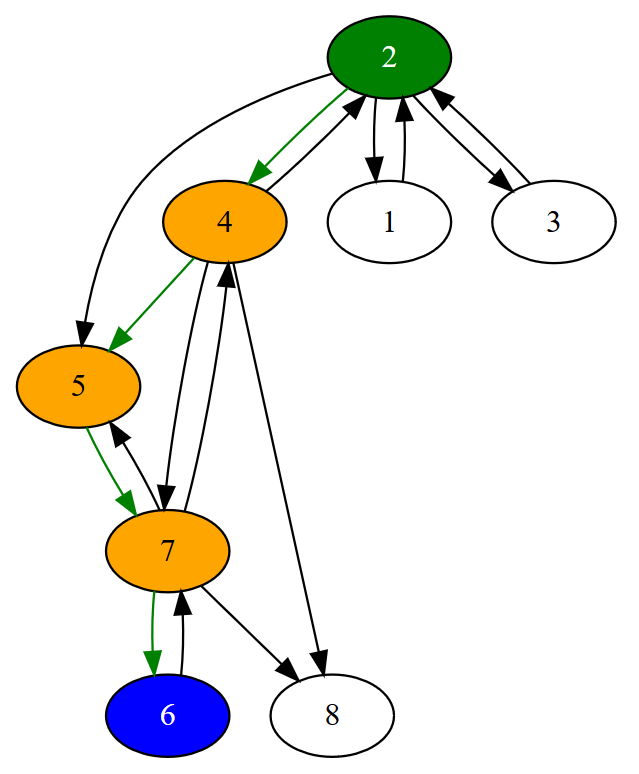
\includegraphics[width=\linewidth]{groundplan_msk_simple_graph}
		\caption{Path tracking using a graph. A green node marks the path's start, orange nodes the visited rooms, and blue the last node that was visited. Edges in green help visualize the path and the order which it was travelled.}
		\label{fig:groundplan_msk_simple_graph}
	\end{figure}


	
	\section{Results}
\label{sec:results}
This section describes the experimental results of the final recognition system. It includes the performance of the individual steps: painting segmentation, the matching algorithm and room localization. 


\subsection{Dataset}
The main dataset consists of 688 pictures of all art items in the museum which functions as a database. These pictures are taken at eye-level height and each picture contains one or multiple art items. One part of the dataset is taken with a Nokia 7 Plus camera, which offers a base resolution of 3024 by 4032 pixels and the other part is taken with a Samsung A3 2016, which offers a base resolution of 3096 by 4128 pixels. All pictures in the dataset are compressed to 1000 x 1000 pixels. To reduce the load time of this dataset, a prebuilding stage was implemented. This stage reduces each image to a collection of interest points and corresponding descriptors for these interest points as generated by the ORB \cite{Rublee2011} algorithm. 

\subsection{Test set}
Apart from the dataset, two different testing sets exist to evaluate the algorithm. The first testing contains still images of various shots at the museum. This dataset contains more difficult examples such as steep angles or hard to detect paintings. A random sample ($n = 30$) was selected and labeled manually. This first test set is used to evaluate the segmentation and matching part. A second testing set are various videos which emulates a person recording paintings while moving trough the museum. Similar to the first test set, a small segment (1 minute) of the video was taken and labeled manually. The video test set has the added disadvantage of motion blur, decreasing the effectiveness of segmentation and matching.


\subsection{Segmentation Accuracy}
The random sample from the test set was first manually segmented to indicate a perfect segmentation. This results in 4 coordinates of a polygon which represent the ideal polygon. Afterwards, the segmentation is done automatically by the algorithm, which also gives four coordinates of a polygon. To illustrate, both polygons are shown on figure \ref{fig:painting_segmentation_validation_1}.
To measure the similarity of these two polygons, and thus the correctness of the segmentation, we first calculate the intersection area $A_i$ and the area of the ideal polygon $A_{pi}$. The ratio of $A_i$ to $A_{pi}$ describes the closeness of two polygons with 100\% being a perfect match and 0\% meaning there is no intersection at all between the two polygons. There is one case where this statistic does not work. When the ideal polygon is fully enclosed by the predicted polygon, $A_i$ will be equal to $A_{pi}$, resulting in a fake perfect match. To prevent this, the roles of the green and red polygon are switched such that we now consider the area of the predicted polygon, $A_{pp}$, instead of $A_{pi}$.
\begin{figure}
	\centering
	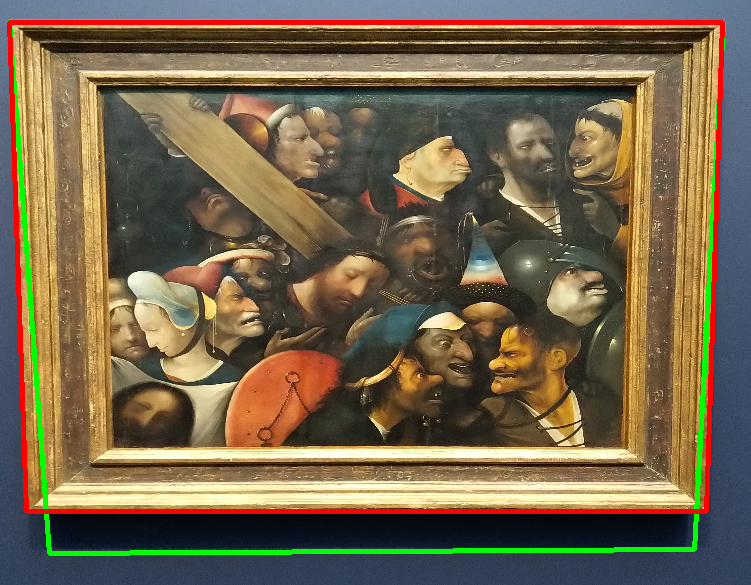
\includegraphics[width=\linewidth]{painting_segmentation_validation_1}
	\caption{A comparison of a manually selected polygon (red) and the polygon found by the segmentation algorithm (green).}
	\label{fig:painting_segmentation_validation_1}
\end{figure}


Using this metric, the segmentation method achieves a 47.10\% average correctness score. Figure \ref{fig:segmentation_correctness_graph} shows the overall results. There are three reasons for this score. The first reason is the way the ground truth is established. Figure \ref{fig:reason_bad_segmentation} shows the actaul painting segment, surrounded by a red polygon, and the predicted painting segment, surrounded by a green polygon. Due to the use of the Canny edge detector and choosing the outermost contours that are found, a painting frame will almost always be included as part of the painting, resulting in a lower total score. The second reason is due to shadows. Figure \ref{fig:negative_case_shadow} shows how a shadow extends below the painting frame. The shadow and background wall differ in color intensity, resulting in an edge from the Canny edge detector. These edges extend the painting frames and because the contour with the largest area is sought after, the segmentation step will include the shadow as part of the painting in all cases. A third reason occurs when the full painting frame is not visible. In this case, a contour is likely to be not found, resulting in no segmentation at all.


\begin{figure}
	\centering
	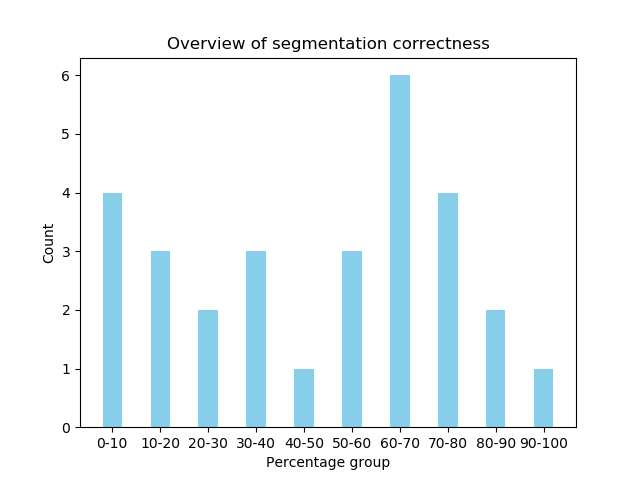
\includegraphics[width=\linewidth]{segmentation_correctness_graph}
	\caption{The results of the segmentation step using the area method. For example, 6 paintings got an area overlap between 60 and 70 percent.} 
	\label{fig:segmentation_correctness_graph}
\end{figure}
\begin{figure}
	\centering
	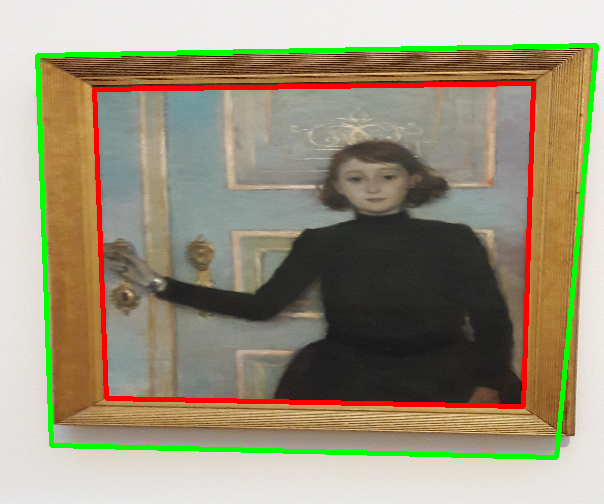
\includegraphics[width=\linewidth]{reason_bad_segmentation}
	\caption{Example of the ground truth (red polygon) versus the predicted polygon (green polygon). Due to the Canny edge detection and choosing outer contours, the frame edge will almost always be included as part of the painting.}
	\label{fig:reason_bad_segmentation}
\end{figure}



\begin{figure}
	\centering
	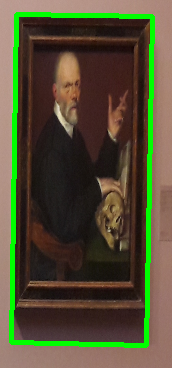
\includegraphics[width=0.5\linewidth]{negative_case_shadow}
	\caption{An example of a shadow underneath the painting. This usually results in the segmentation algorithm to include this shadow as part of the painting because of the strong edge.}
	\label{fig:negative_case_shadow}
\end{figure}


\subsection{Matching and Localization Accuracy}
The matching algorithm has to be evaluated manually by comparing the matcher's result against each image in the test set. The correctness of the matching algorithm is simply the ratio of the correct matches against the false matches. Here it is found that 46.7\% of paintings are matched correctly. Due to this rather bad result, the localisation method fails. More than half of the matched paintings are wrong, resulting in jumps between different rooms that are not logical. The localisation part of this algorithm is therefore not trustworthy  to be used.




\subsection{Qualitative analysis}
In this subsection, we will present a qualitative analysis of our algorithm. We will discuss its strengths, flaws and, with each point, present an example case to help as a visual aid. The flaws in particular help paint a picture of what can be done better in a future iteration of the algorithm. 


One of the algorithm's major strengths lies in its simplicity. The block diagram shows a very linear approach to the problem with concrete begin- and endpoints. Though machine learning is often used in the field of computer vision and has a lot of benefits, the algorithm does not employ it. We do not deny its usefulness and believe that it may be beneficial to implement it in a future version of the algorithm. The classification of pixels may be one of the problems tackled as a way of assisting the segmentation. Even though the algorithm's simplicity is presented as one of its strengths, it can also be considered as one of its weaknesses, much like a double-edged sword.


Furthermore, the algorithm works relatively fast for matching and determining the location of a potential user using a single image. When taking the average of 30 runs of the algorithm with a frame, we get a time of $0.78\pm0.01 s$. Even though this is nearing almost a second, it is important to note that it is expected to take some time to complete as the dataset being matched against is quite large. This will be discussed more in depth further below.


In addition, the use of ORB causes the results of each program run to be invariant given the same input image, implying a deterministic nature. This is of course on the premise that certain parameters such as the Canny thresholds remain the same between runs. Figure \ref{fig:double} shows how two images have the same match and detected keypoints between two runs. However, due to not detecting different potential candidate matches between runs results in the algorithm never being able to present a different solution for the given image.


On top of that, the algorithm is resilient when it can not successfully segment an image. The default behavior is trying to find a frame, extract it, and using it as the input of the matching stage of the algorithm. If no frame can be found, rather than ignoring the current video frame or image, we supply the entire thing to be matched. This may slow the matching stage down by a small margin but has the benefit of still being able to spit out a potential positive match. Figure \ref{fig:full_frame} shows an example where an entire frame is supplied to the matching function, but still manages to find a correct match. This resiliency comes at a price. The matching phase performs slightly worse, as the frame may contain additional features that can help with matching a painting. Should this algorithm be used in an actual application, this can occur when the user is standing too close to a painting. 


As was hinted in the previous point, supplying a full frame or image to the matching phase may slow things down. The input image's size definitely affects the time needed to complete in a negative way. Therefore, images used for the segmentation and matching phases are resized to between \verb|25%-50%| their original size. This may result in some loss of precision but should not affect the overall efficiency of the algorithm. Table \ref{tab:quadratic} shows that resizing an image from the query set to a quarter of its size quadratically decreases the amount of pixels needed to evaluate. The same resizing is applied to the building stage of the database.

\begin{table}[]
	\centering
	\begin{tabular}{rcccl}
		\multicolumn{1}{l}{} & \textbf{Width} & \textbf{Height} & \textbf{Total pixels} &  \\
		\textbf{Original}    & 2322           & 128            & 9 585 216             &  \\
		\textbf{Resized}     & 580.5          & 1032            & 599 076               & 
	\end{tabular}
	\caption{Taking a 9.5 megapixel picture and resizing it to a quarter of its original size results in a decrease of total pixels by a factor of 16}
	\label{tab:quadratic}
\end{table}

Another problem arises due to an assumption in the matching stage. A match is determined by the smallest sum of distances calculated over the matches between two images. This assumption works well when the amount of matches is fixed between every match between the query image and the training set. ORB detects keypoints and associates descriptors up to a maximum of 200. But what if it can not detect a lot of keypoints, maybe even none? Figure \ref{fig:flat_surface} shows how paintings that have a relative 'flat' surface without discerning features (sometimes even to the naked eye) have trouble being matched to a picture in the data set. Suppose that the segmentation phase detects such a painting and supplies it to the matching phase. A cascade of erroneous matches and room localizations may occur. The inverse is also true, as having an entry in the data set with few keypoints can result in a painting with many keypoints being wrongfully matched with a 'flat' one.


Figure \ref{fig:smaller_rectangle} shows the flaws of the segmentation phase. If no quad can be approximated from the painting then there is a chance that polygons with a smaller surface area may be erroneously detected and fed to the matching stage. The problem lies in the combination of using the Canny operator along with the approximation of quad polygons. Our algorithm is unable to deal with 'valid' paintings that have an approximated polygon with an amount of sides higher than 4.


The final major flaw that will be presented lies in the matching phase: matching a painting is done by doing a linear lookup in the database. For a single image this does not pose that much of a problem. The same can not be said when we expanded our algorithm to analyze the frames of a video. This slowdown is mitigated through two changes to the original algorithm. First, we run it only every 30 video frames which is equivalent to around 1 second in real life. Second, the algorithm offloads the matching procedure to a multi-threading environment, freeing the video code from freezing. But what causes this in the first place? 


Considering there are 688 pictures in the database, coupled with the keypoints and descriptors that were extracted during the prebuilding phase, are matched with the descriptors of the segmented painting results in a total. In our solution, we limit the amount of keypoints and descriptors by 200, which still results in 27 520 000 elements needing to be compared to during each matching phase. Another problem lies in the use of the brute force matching, which tries to compare the keypoints and descriptors of the segmented painting with this dataset. Our original design of this algorithm anticipated that a linear lookup would not pose a problem for our assumed small database of 688 paintings. Szeliski \cite{Szeliski2010} suggests that a linear lookup has $O(n^{2})$ behavior as the database starts to grow. Our algorithm seems to prove this suggestion. A future iteration of this algorithm may need to place the focus on this part of the algorithm.


\begin{figure}
	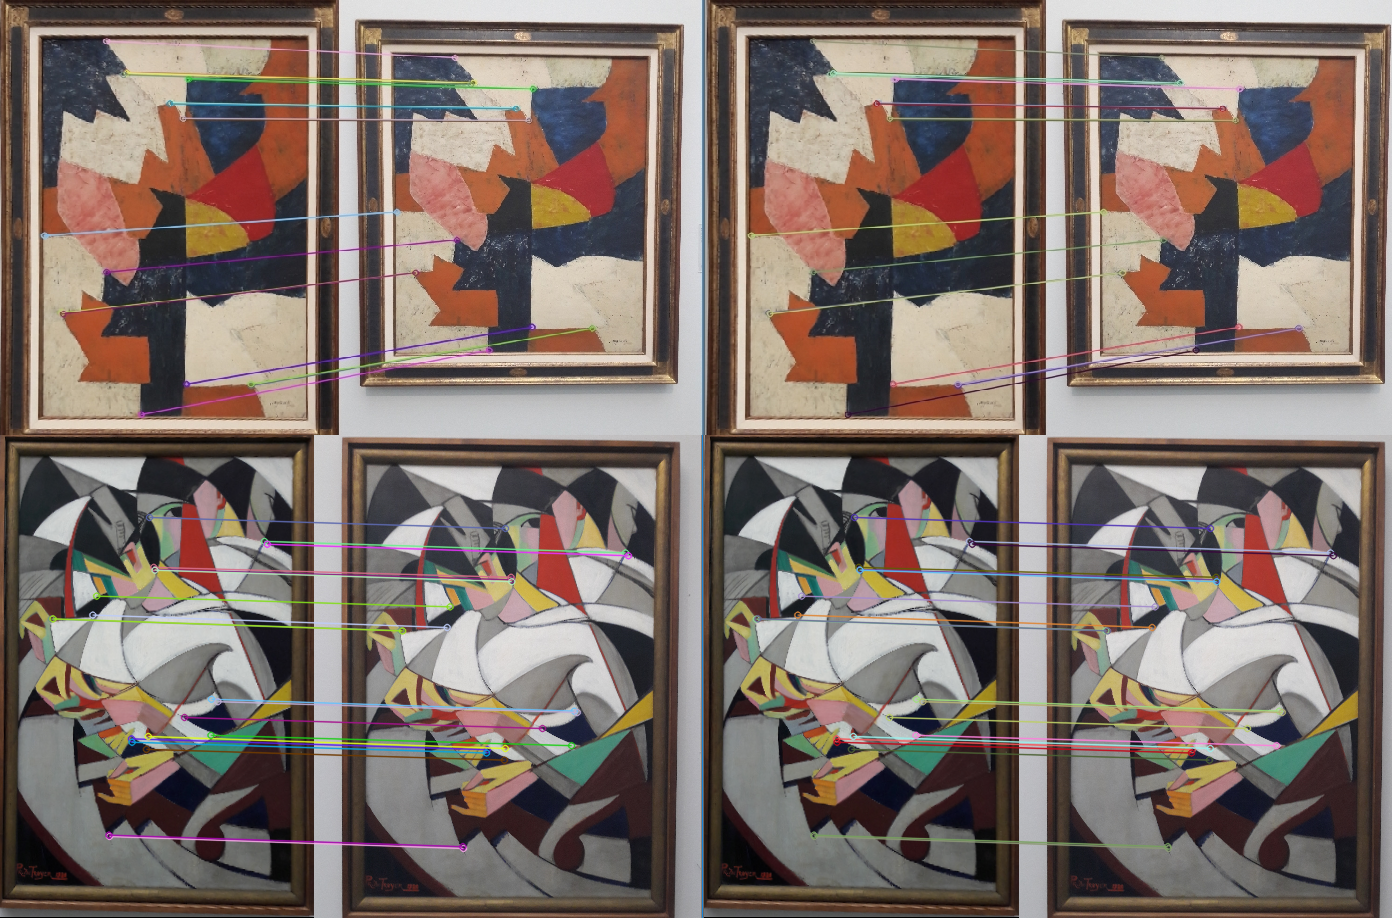
\includegraphics[width=\linewidth]{double}
	\caption{Two different extracted paintings being matched with the database show that with the same Canny thresholds the same match will be returned}
	\label{fig:double}
\end{figure}

\begin{figure}
	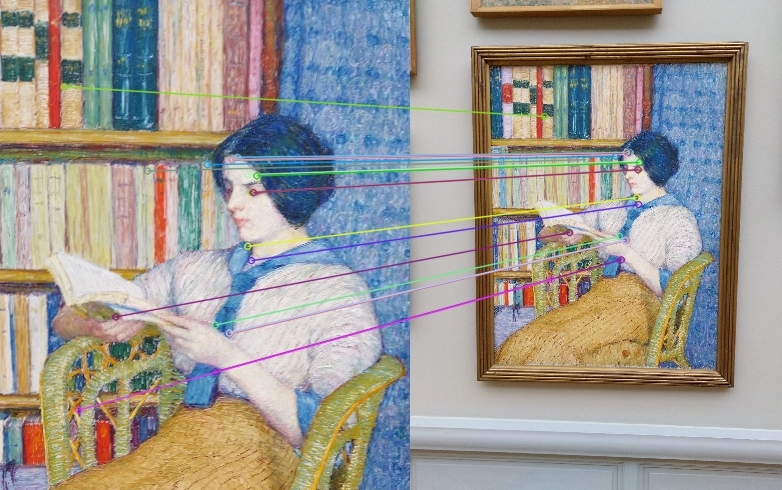
\includegraphics[width=\linewidth]{full_frame}
	\caption{Matching of an entire frame or a closeup of a painting may still yield a correct match}
	\label{fig:full_frame}
\end{figure}

\begin{figure}
	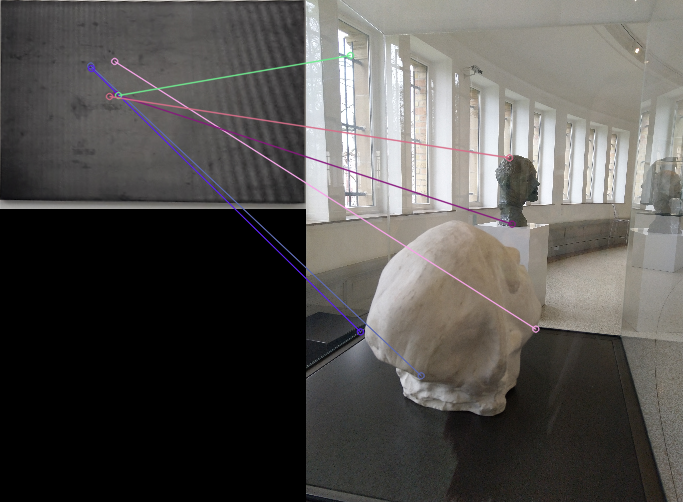
\includegraphics[width=\linewidth]{flat_surface}
	\caption{The extracted painting from the frame is grayish and looks 'flat'. There are not many keypoints that can be detected and successfully matched in this case resulting in a false overall match.}
	\label{fig:flat_surface}
\end{figure}

\begin{figure}
	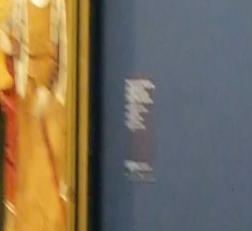
\includegraphics[width=\linewidth]{smaller_rectangle}
	\caption{Information about the paintings hanging next to them have a polygonal shape and may be extracted erroneously}
	\label{fig:smaller_rectangle}
\end{figure}
	\section{Conclusion}
\label{sec:conclusion}
In this work we discussed three parts: a painting segmentation technique, a matching technique and the localisation method. Painting segmentation is achieved using a Canny edge detection combined with finding contours. Due to canny edge detection, frames are also included as part of the painting. The extracted paintings are supplied to a brute-force ORB matcher which detects key features and descriptors from the paintings. The matching happens in a linear fashion, resulting in a slow execution speed, which was solved using multi-threading and reducing the dataset size. Both the segmentation and matching are subpar, scoring respectively 47.10\% and 46.7\% accuracy. Due to this low accuracy, the localisation step is deemed not trustworthy to be used.

The current implementation of the algorithm uses a per-frame matching technique. Using a buffer and applying e.g. majority voting or weighted voting could increase the accuracy of the matching method. 



	\bibliographystyle{IEEEtran}
	\bibliography{IEEEabrv,library}
\end{document}